\section{Background}
    \subsection{Stato dell'arte}

      \begin{frame}{\insertsectionhead}{\insertsubsectionhead}
        \begin{columns}
          \begin{column}{.7\textwidth}
            \begin{block}{Programmazione aggregata}
              La programmazione aggregata costituisce un'alternativa all'approccio ``classico'' volta a semplificare la progettazione, creazione e manutenzione di sistemi distribuiti complessi.
            \end{block}

            \begin{block}{Linguaggi}
              I principali linguaggi di programmazione aggregata sono:

              \begin{itemize}
                \item ScaFi
                \item Protelis
              \end{itemize}
            \end{block}
          \end{column}
          \begin{column}{.25\textwidth}
            \begin{figure}
              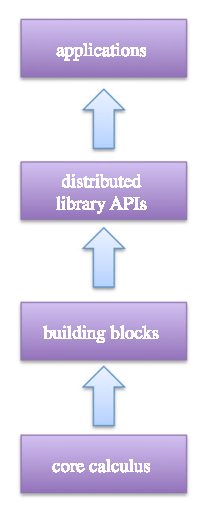
\includegraphics[height=.7\textheight]{res/fig/stack-partial.eps}
            \end{figure}
          \end{column}
        \end{columns}
      \end{frame}

      \begin{frame}{\insertsectionhead}{\insertsubsectionhead}
        \begin{columns}
          \begin{column}{.8\textwidth}
            \begin{block}{Protelis}
              \begin{itemize}[<+->]
              \item
                  Linguaggio di programmazione basato sul paradigma aggregato fortemente influenzato da \emph{Proto}
                \item
                  Incorpora le principali funzionalità di computazione spaziale della programmazione aggregata
                \item
                  Possiede una sintassi più simile ai linguaggi strutturati tradizionali come C o Java
                \item
                  È \emph{Java-hosted}
                  \begin{itemize}
                    \item richiede un ambiente JVM in cui eseguire l'interprete
                  \end{itemize}
              \end{itemize}
            \end{block}
          \end{column}
          \begin{column}{.15\textwidth}
            \begin{figure}
              
\includegraphics[width=\textwidth]{../res/fig/protelis-logo.png}
            \end{figure}
          \end{column}
        \end{columns}
      \end{frame}

    \subsection{Problematica}

    \begin{frame}{\insertsectionhead}{\insertsubsectionhead}
      \begin{columns}
        \begin{column}{.6\textwidth}
          \begin{alertblock}{\insertsubsectionhead}
            \begin{itemize}
              \item<1->
                Il linguaggio richiede una rete di dispositivi su cui eseguire:
                \begin{itemize}
                  \item<2-> rete fisica
                  \item<3-> NASA WorldWind
                  \item<4-> ProtelisVM
                  \item<5-> Alchemist
                \end{itemize}
            \end{itemize}
          \end{alertblock}
        \end{column}
        \begin{column}{.35\textwidth}
          \begin{figure}
            \centering
            \includegraphics<2>[width=.85\textwidth]{res/fig/network.png}
            \includegraphics<3 | handout 0>[width=.85\textwidth]{res/fig/nasaworldwind.png}
            \includegraphics<4 | handout 0>[width=.85\textwidth]{res/uml/protelis-vm.eps}
            \includegraphics<5 | handout 0>[width=.85\textwidth]{res/fig/alchemist.png}
            \includegraphics<6 | handout 0>[width=.85\textwidth]{res/fig/protelis-alchemist-arch.eps}
          \end{figure}
        \end{column}
      \end{columns}
    \end{frame}

    \subsection{Requisiti e casi d'uso}

    \begin{frame}{\insertsectionhead}{\insertsubsectionhead}
      \begin{columns}
        \begin{column}{.5\textwidth}
          \begin{block}{Requisiti}
            \begin{itemize}
              \item
                Progettare un sistema che permetta di iniziare a utilizzare Protelis senza configurazioni
                \begin{itemize}
                  \item nessun build-script
                  \item nessun deploy di dispositivi
                \end{itemize}
              \item
                L'utente si assume essere inesperto della piattaforma
                \begin{itemize}
                  \item l'interfaccia deve essere semplice e immediata
                \end{itemize}
              \item La piattaforma dovrebbe essere accessibile tramite browser
            \end{itemize}
          \end{block}
        \end{column}
        \begin{column}{.45\textwidth}
          \begin{figure}
            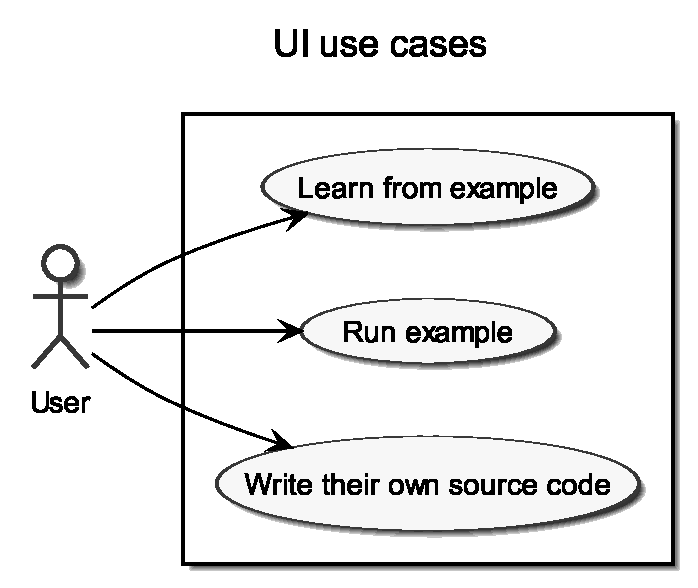
\includegraphics[width=\textwidth]{res/uml/use-cases-frontend.eps}
          \end{figure}
        \end{column}
      \end{columns}
    \end{frame}

    \begin{frame}{\insertsectionhead}{\insertsubsectionhead}

      \begin{block}{Analisi del problema}
        \begin{itemize}
          \item
            non è possibile eseguire un interprete Protelis all'interno della sandbox un browser
            \begin{itemize}
              \item le Java applet sono deprecate da tempo
            \end{itemize}
          \item
            è necessario suddividere l'architettura in due componenti
            \begin{itemize}
              \item un server che espone API per l'esecuzione del codice
              \item un'interfaccia Single-Page accessibile tramite browser
            \end{itemize}
        \end{itemize}
      \end{block}

      \begin{figure}
        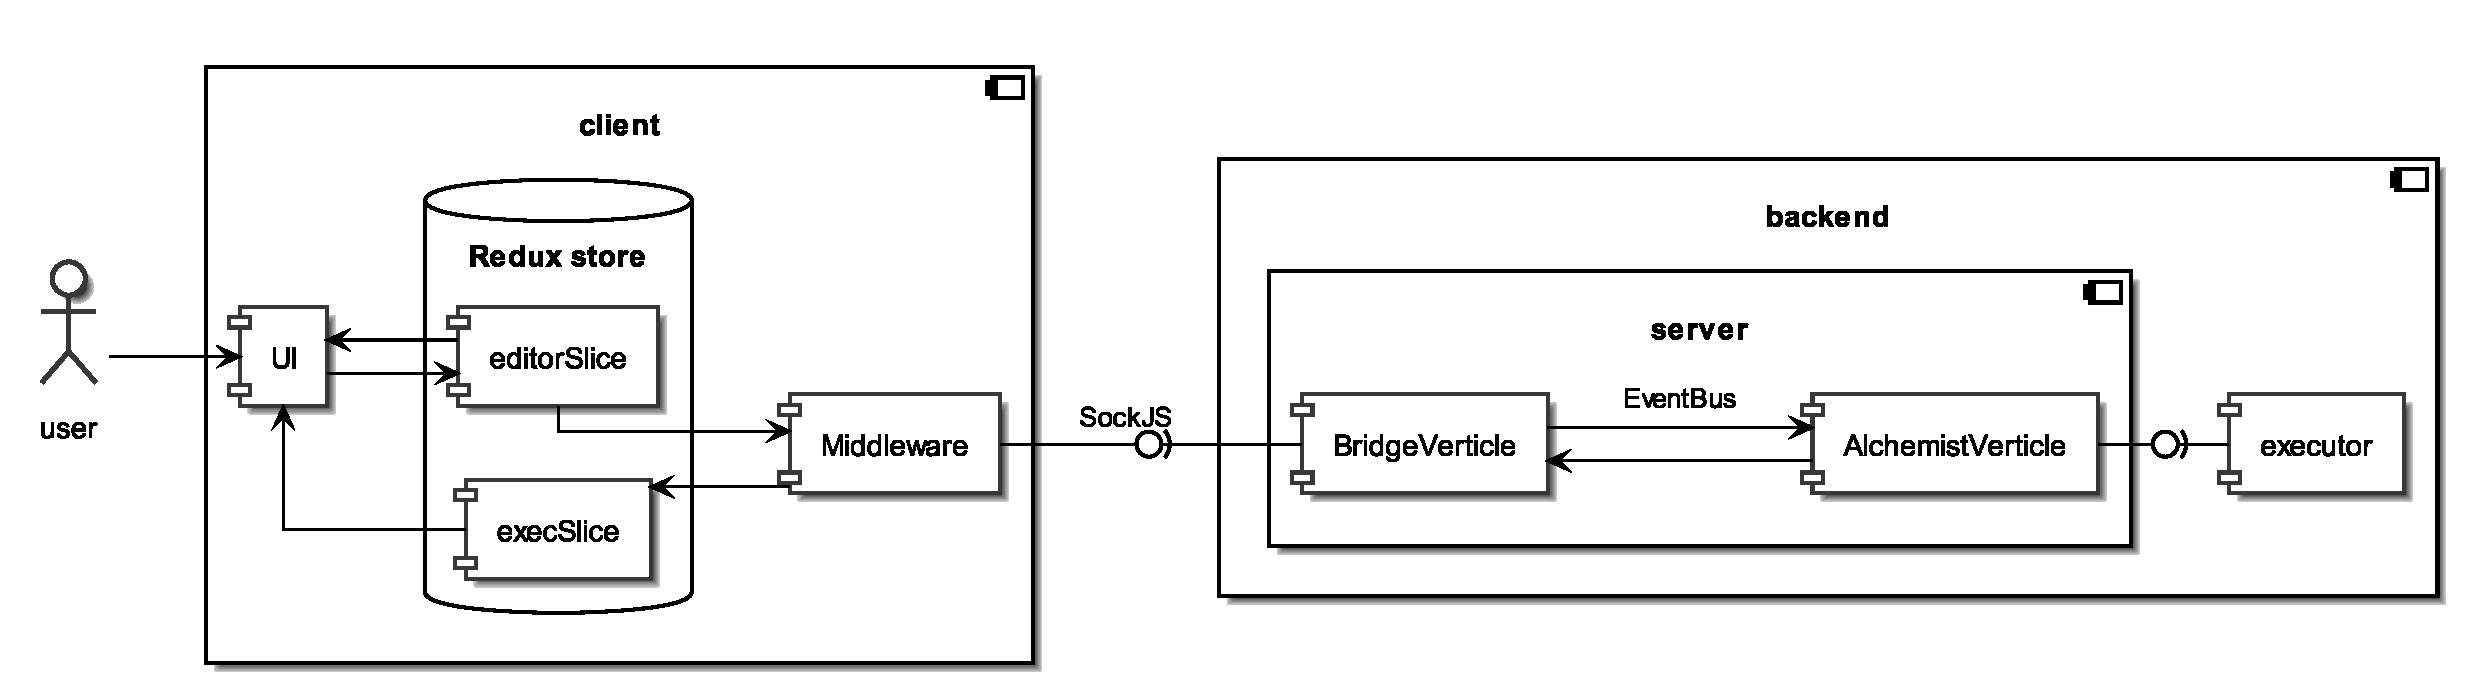
\includegraphics[width=.71\textwidth]{../res/uml/architecture-design.eps}
      \end{figure}
    \end{frame}
